%\documentclass[runningheads]{llncs}
\documentclass{llncs}
%\usepackage{graphicx}
\usepackage{xcolor}
\usepackage{amssymb}
\usepackage{dsfont}
\usepackage{amsmath} 

\usepackage{url}
\usepackage{cancel}
\usepackage{verbatim}
\usepackage{alltt}
\usepackage{graphicx}
\usepackage{prooftree}

\usepackage{latexsym}
\usepackage{xspace}
%\usepackage{draft} REVOIR
\usepackage{comment}
%\usepackage{ntheorem}
%\usepackage{amsthm} % \proof seems to exist in llncs

\newcommand{\revoir}[1]{\mbox{{[*** {\bfseries\large #1} ***]}}}
\newcommand{\nouveau}[1]{\textcolor{blue}{#1}}

\newcommand{\egdef}%
   {\ensuremath{\:\mathrel{\raisebox{-.7ex}%
   {$\stackrel{\rm def}{=\mkern-8mu=}$}}\:}}

\newcommand{\simlight}{\texttt{simlight}\xspace}

\newtheorem{Prog}{Program}
%\newcommand{\idcoq}[1]{\texttt{#1}}
\newcommand{\idcoq}[1]{\ensuremath{\mathit{#1}}}
\newcommand{\impl}{\ensuremath{\Rightarrow}}
\newcommand{\flequiv}{\ensuremath{\leftrightarrow}}
\newcommand{\todo}[1]{\textcolor{blue}{\textsc{[#1]}}}
\newcommand{\XM}[1]{{\color{red} #1}} % Xiaomu's editing
\newcommand{\JFM}[1]{{\color{red} #1}} % JF's editing

% BEGIN For coqdoc 

\newenvironment{coqdoccode}{}{}

\newlength{\coqdocbaseindent}
\setlength{\coqdocbaseindent}{0em}

\newcommand{\coqdef}[3]{#3}
\newcommand{\coqref}[2]{#2}
\newcommand{\coqexternalref}[3]{#3}

% Beginning of a line without any Coq indentation
\newcommand{\coqdocnoindent}{\noindent\kern\coqdocbaseindent}
% Beginning of a line with a given Coq indentation
\newcommand{\coqdocindent}[1]{\noindent\kern\coqdocbaseindent\noindent\kern#1}
% End-of-the-line
\newcommand{\coqdoceol}{\hspace*{\fill}\setlength\parskip{0pt}\par}
% Empty lines (in code only)
\newcommand{\coqdocemptyline}{\vskip 0.4em plus 0.1em minus 0.1em}

% own name
\newcommand{\coqdoc}{\textsf{coqdoc}}

% pretty underscores (the package fontenc causes ugly underscores)
%BEGIN LATEX
\def\_{\kern.08em\vbox{\hrule width.35em height.6pt}\kern.08em}
%END LATEX

% macro for typesetting keywords
\newcommand{\coqdockw}[1]{\texttt{#1}}

% macro for typesetting variable identifiers
\newcommand{\coqdocvar}[1]{\textit{#1}}

% macro for typesetting constant identifiers
\newcommand{\coqdoccst}[1]{\textsf{#1}}

% macro for typesetting module identifiers
\newcommand{\coqdocmod}[1]{\textsc{\textsf{#1}}}

% macro for typesetting module constant identifiers (e.g. Parameters in
% module types)
\newcommand{\coqdocax}[1]{\textsl{\textsf{#1}}}

% macro for typesetting inductive type identifiers
\newcommand{\coqdocind}[1]{\textbf{\textsf{#1}}}

% macro for typesetting constructor identifiers
\newcommand{\coqdocconstr}[1]{\textsf{#1}}

% macro for typesetting tactic identifiers
\newcommand{\coqdoctac}[1]{\texttt{#1}}

% These are the real macros used by coqdoc, their typesetting is 
% based on the above macros by default.

\newcommand{\coqdoclibrary}[1]{\coqdoccst{#1}}
\newcommand{\coqdocinductive}[1]{\coqdocind{#1}}
\newcommand{\coqdocdefinition}[1]{\coqdoccst{#1}}
\newcommand{\coqdocvariable}[1]{\coqdocvar{#1}}
\newcommand{\coqdocconstructor}[1]{\coqdocconstr{#1}}
\newcommand{\coqdoclemma}[1]{\coqdoccst{#1}}
\newcommand{\coqdocclass}[1]{\coqdocind{#1}}
\newcommand{\coqdocinstance}[1]{\coqdoccst{#1}}
\newcommand{\coqdocmethod}[1]{\coqdoccst{#1}}
\newcommand{\coqdocabbreviation}[1]{\coqdoccst{#1}}
\newcommand{\coqdocrecord}[1]{\coqdocind{#1}}
\newcommand{\coqdocprojection}[1]{\coqdoccst{#1}}
\newcommand{\coqdocnotation}[1]{\coqdockw{#1}}
\newcommand{\coqdocsection}[1]{\coqdoccst{#1}}
\newcommand{\coqdocaxiom}[1]{\coqdocax{#1}}
\newcommand{\coqdocmodule}[1]{\coqdocmod{#1}}

% END For coqdoc 

% macros for this paper
\newcommand{\diag}{\coqdocvar{diag}\xspace}
\newcommand{\inversion}{\coqdoctac{inversion}\xspace}
\newcommand{\inv}{\coqdoctac{inv}\xspace}
\newcommand{\casetac}{\coqdoctac{case}\xspace}
\newcommand{\match}{\coqdoctac{match}\xspace}
\newcommand{\with}{\coqdoctac{with}\xspace}
\newcommand{\intac}{\coqdoctac{in}\xspace}
\newcommand{\retac}{\coqdoctac{return}\xspace}
\newcommand{\refine}{\coqdoctac{refine}\xspace}
\newcommand{\Prop}{\coqdockw{Prop}\xspace}
\newcommand{\True}{\coqdocvar{True}\xspace}
\newcommand{\eveni}{\coqdocvar{even\_i}\xspace}
\newcommand{\EZ}{\coqdocvar{E0}\xspace}
\newcommand{\ET}{\coqdocvar{E2}\xspace}
\newcommand{\evenf}{\coqdocvar{even\_f}\xspace}
\newcommand{\prone}{\coqdocvar{pr\_1}\xspace}
\newcommand{\prET}{\coqdocvar{premises\_E2}\xspace}
\newcommand{\EXPR}{\coqdocvar{EXPR}\xspace}
\newcommand{\PROOFEV}{\coqdocvar{PROOF\_EV}\xspace}
\renewcommand{\PROOFEV}{\mathit{PE}}

% For automated inclusion of .tex files generated from coqdoc
\newcommand{\coqdocinput}[1]{\input{#1}}

\newcommand{\union}{\ensuremath{\cup}}

\newenvironment{ml}
  {\begin{alltt}
   \footnotesize} %% 3.12.0
  {\end{alltt}
  }

\newenvironment{coq}
  {\begin{alltt}
   \footnotesize} %% 8.3pl2 (April 2011)
  {\end{alltt}
  }

\newenvironment{humC}
  {\begin{alltt}
   \footnotesize}
  {\end{alltt}
  }



\begin{document}

\title{Scaling up Small Inversions
}
\titlerunning{Scaling up Small Inversions}
% Official order as registered at CPP
\author{Jean-Fran\c{c}ois Monin\inst{1,2}
\and 
Xiaomu Shi\inst{1}
}
\institute{%
Universit\'{e} de Grenoble 1 - LIAMA
\and CNRS - LIAMA
}
\authorrunning{J.-F. Monin, X. Shi}

\maketitle

\begin{abstract}
  When reasoning on formulas involving large-size inductively defined
  relations, such as the semantics of a real programming language,
  many steps require the inversion of a hypothesis. The built-in
  "inversion" tactic of Coq can then be used, but it suffers from
  severe controllability and efficiency issues.  A proof-trick called
  small inversions by one of the co-authors provides a part of the
  solution. It is based on a suitable diagonal auxiliary
  predicate. However, many important practical situations are not
  covered by this technique.  We present here an improvement inspired
  by the impredicative encoding of inductive data-structures. Our
  experiments in the SimSoC-Cert project show that this technique
  successfully scales up to proofs of non-trivial programs according
  to the operational semantics of C as defined in Compcert.
\end{abstract}



%-------------------------------------------------------------------------
\section{Introduction}
\label{sec:intro}

\subsection{Simulation of Systems-on-Chip}

Systems-on-Chip (SoC), used in devices such as smart-phones, contain both
hardware and software. A part of the software is generic and can be used with
any hardware systems, and thus can be developed on any computer. In contrast,
developing and testing the SoC-specific code can be done only with this SoC, or
with a \emph{software executable model} of the SoC. 
To reduce the time-to-market, the software development must start
before the hardware is ready. Even if the hardware is available,
simulating the software on a model provides more debugging
capabilities.
%
The %most abstract and 
fastest simulators use native simulation.
%
The software of the \emph{target} system (i.e., the SoC) is compiled with
the normal compiler of the computer running the simulator, 
but linked with special system
libraries. Examples of such simulators are the Android and iOS
SDKs.

In order to develop low-level system code, one needs a simulator that
can take the real binary code as input. Such a simulator requires a
model of the processor and of its peripherals (such as UART, DMA,
Ethernet card, etc). When simulating a smart-phone SoC, this kind of
functional simulator can be from 1 to 100 times slower than the real
chip.
%
These simulators have other uses, for example, as
reference models for the hardware verification.
An error in the simulator can then mislead both the software and the hardware
engineers.
QEMU~\cite{qemu} is an open-source processor emulator
coming with a set of device models; it can simulate several
operating systems. Other open-source simulators include
UNISIM~\cite{unisim} (accurately-timed)
and
SimSoC~\cite{ossc09}, developed by some colleagues, %at LIAMA 
which is loosely-timed (thus faster).
Simics~\cite{simics} is a commercial alternative.
%
The usual language to develop such simulators is C++, combined with
the SystemC~\cite{systemc-lrm} and OSCI-TLM~\cite{tlm-osci}
libraries.

\medskip
The work reported here is related to SimSoC.

\subsection{The Need for Certification}

Altogether, a functional simulator is a complex piece of software.
SimSoC, which is able to simulate Linux both on ARM and PowerPC
architectures at a realistic speed
(over 10 Millions of instructions per second per individual core), 
includes about 60,000 lines of C++
code. The code uses complex features of the C++ language and of the
SystemC library. Moreover, achieving high simulation speeds requires
complex optimizations, such as dynamic translation~\cite{qemu}.

This complexity is problematic, because beyond speed,
\emph{accuracy} is required:
all instructions have to be simulated
exactly as described in the documentation.
There is a strong need to strengthen the confidence that
simulations results match the expected accuracy. 
Intensive tests are a first answer.
For instance, as SimSoC is able to run a Linux kernel
on top of a simulated ARM, we know that many situations are covered.
However it turned out, through further experiments, that it was not
sufficient: wrong behaviors coming from rare instructions
were observed after several months.
%
Here are the last bugs found and fixed by the SimSoC team while trying to boot
Linux on the SPEArPlus600 SoC simulator.
\begin{itemize}
\item After the execution of an \texttt{LDRBT} instruction, the contents of the
  base register (\texttt{Rn}) was wrong. It was due to a bug in the reference
  manual itself; the last line of the pseudo-code has to be deleted.
\item After a data abort exception, the base register write-back was not
  canceled.
\item Additionally, a half-word access to an odd address while
  executing some SPEArPlus600 specific code was not properly handled. 
\end{itemize}

Therefore we propose here to certify the simulator,
that is, to prove, using formal methods --
here: the Coq proof assistant \cite{coqmanual,coqart} --
that it conforms to the expected behavior.

This is a long term goal.
Before going to the most intricate features of a simulator such as SimSoC,
basic components have to be considered first.
We then decided to focus our efforts on a sensible and important 
component of the system: the CPU part of the ARMv6 architecture 
(used by the ARM11 processor family).
%
This corresponds to a specific component of the SimSoC simulator,
which was previously implementing the ARMv5 instruction set only.
Rather than certifying this component, it seemed to us more feasible
to design a new one directly in C, in such a way that it can be
executed alone, or integrated in SimSoC (by including the C code in
the existing C++ code).
%
We call this new component \simlight \cite{rapido11}. Combined with a small
\texttt{main} function, \simlight can simulate ARMv6 programs as long
as they do not access any peripherals (excepted the physical memory)
nor coprocessors. There is no MMU (Memory Management Unit) yet. Integrating it in SimSoC just
requires to replace the memory interface and to connect the interrupts
(IRQ and FIQ) signals.

\smallskip
The present paper reports our first efforts 
towards the certification of \simlight.
We currently have a formal description of the ARMv6 architecture,
a running version of \simlight,
and we are in the way of performing correctness proofs.
The standard way for doing this is to use Hoare logics
or a variant thereof.
Various tools exist in this area, 
for example Frama-C \cite{frama-c}.
We chose to try a more direct way,
based on an operational semantics of C;
more precisely the semantics of Compcert-C defined in the Compcert project
\cite{Leroy-Compcert-CACM}.
One reason
is that we look for a tight control on the formulation of proof obligations
that we will have to face.
Another advantage is that we can consider the use of
the certified compiler developed in Compcert,
and get a very strong guarantee on the execution of 
the simulator (but then, sacrificing speed to some extent\footnote{%
According to our first experiments, \simlight compiled with Compcert
is about 50~\% to 70~\% slower than \simlight compiled with \texttt{gcc -O0}.
%It is indeed interesting : by running natively without any simulation, 
%we got a faster executable with Compcert~!
}).

Another interesting feature of our work is that 
the most tedious (hence error prone) part of the formalization --
the specification of instructions --
is automatically derived from the reference manual.
It is well known that the formal specification of such big applications
is the main weak link in the whole chain.
Though our generators cannot be proved correct, because the statements
and languages used in the reference manual have no formal semantics,
we consider this approach as much more reliable than a manual formalization.
Indeed, a mistake in a generator will impact several or all operations,
hence the chances that it will be detected through a visibly wrong behavior
are much higher than with a manual translation,
where a mistake will impact only one (eventually rarely used) operation.

Note that after we could handle the full set of ARM instructions,
our colleagues of the SimSoC team decided to use the same technology
for the SimSoC itself:
the code for simulating instructions in \simlight,
i.e., the current component dedicated to the ARM v6 CPU in SimSoC,
is automatically derived using a variant of our generator,
whereas the previous version for ARM v5 was manually written \cite{rapido11}.


Fig.~\ref{fig:archi} describes the overall architecture. 
The contributions of the work presented in this paper are 
the formal specification of the ARMv6 instruction set
and the correctness proof of a significant operation.
More precise statements on the current achievements 
are given in the core of the paper.
 
\smallskip
\emph{Related Work.}
A fully manual formalization of the fm8501 and ARMv7 architectures are reported
in \cite{fm8501} and \cite{FoxM10}. 
The formal framework is respectively ACL2 and HOL4 instead of Coq, 
and the target is to prove that the hardware or microcode implementation of 
ARM operations are correct wrt the ARM specification.
Our work is at a different level:
we want to secure the simulation of programs using ARM operations.
% and no specific target is considered, whereas we are driven by the needs of
% simulation of ARMv6 and 
Another major difference is the use of automatic generation 
from the ARM reference manual in our framework,
as stated above.

\medskip
The rest of the paper is organized as follows.
Section \ref{sec:overallarchi}
presents the overall architecture of \simlight
and indicates for which parts of \simlight 
formal correctness is currently studied.
A informal statement of our current results is also
provided there.
Sections \ref{sec:armmodel} and \ref{sec:simlight}
present respectively our Coq formal reference model of ARM
and the (Coq model of) Compcert-C programs targeted for correctness.
A precise statement of our current results and indications on the proofs are 
given in Section \ref{sec:results}.
We conclude in Section \ref{sec:conclusion} with some hints on
our future research directions.
Some familiarity with Coq is assumed in 
Sections \ref{sec:armmodel}, \ref{sec:simlight} and~\ref{sec:results}.


%%% Local Variables: 
%%% mode: latex
%%% TeX-master: "cpp"
%%% End: 

\section{Auxiliary diagonalization function}
\label{sec:absurd}

We illustrate here the main results of \cite{small_inv}
on the example of even numbers.
Here is the corresponding Coq inductive definition.

\medskip
\coqdocinput{chunk21}
\medskip

\noindent
We see that each rule is given by a constructor in a dependent data type
-- also called an inductive predicate or relation because its sort is \Prop.
Therefore, the elementary way to decompose an object of type \eveni $n$
is to use dependent pattern matching.
This is already done by primitive tactics of Coq
such as \coqdockw{case} and \coqdockw{destruct},
which turn out to be powerful enough in many situations, 
when a condition is satisfied:
the conclusion of the current goal fits all arguments of 
the hypothesis to be analyzed by pattern matching.

Let us first illustrate 
dependent pattern matching on even numbers.
Consider a proof $\PROOFEV$ of type $\eveni\;n$
for some natural number $n$.
For each possible constructor, \EZ or \ET, 
we provide a proof term,
respectively $t_\EZ$ and $t_\ET$.
As usual, this term may depend on the arguments 
of the corresponding constructor,
none for \EZ and, say $x$ and $ex$ for \ET.
More importantly for us, $t_\EZ$ and $t_\ET$ may have
different \emph{types}:
the type $P\;n$ of the whole expression depends on $n$;
in the first branch, the type of $t_\EZ$ is $P\;0$ and
in the second branch, the type of $t_\ET$ is $P\; (S\: (S\:x))$.
Therefore, the syntax of the \coqdockw{match} construct
contains a \coqdockw{return} clause with the expected type
of the result $P\;n$ as an argument;
moreover, 
there is also an \coqdockw{in} clause for the type of $\PROOFEV$
which binds $n$:
% moreover, in order to say where this $n$ comes from,
% there is also an \coqdockw{in} clause for the type of $\PROOFEV$:

\coqdocinput{chunk22}
\medskip

\noindent
Most of the time, Coq users do not need to go to this
level of detail: 
in interactive proof mode, 
if $n$ and $P\;n$ are often clear from the context,
\casetac $\PROOFEV$ will do the job.
More precisely, if we have an hypothesis $H$ of type $\eveni\;n$
and a desired conclusion of type $P\;n$, 
\casetac $H$ will construct a proof term having the previous
shape and answer with two new subgoals:
one for $P\;0$ and one for $P\; (S\: (S\:x))$,
with $\eveni\;x$ as an additional assumption.

More work is needed precisely when there is no obvious relationship
between the conclusion and the hypothesis to be analyzed.
This happens in particular when $H$ is absurd:
the goal should be discharged whatever is its conclusion.
This situation is covered in \cite{small_inv} as follows:
the conclusion is converted 
to an expression \diag $V$,
where $V$ is a value coming from $H$ 
and \diag a suitable diagonal function, such that
the dependent case analysis on $H$ provides only trivial subgoals.
In \cite{small_inv}, we take the type of $H$ itself as a trivial
subgoal but here we will take \True.
For example, assume that we want to conclude
$4=7$ from the hypothesis $H: \eveni\;1$.
Our diagonal function is then defined as follows.

\coqdocinput{chunk24}

\vspace*{-.7\baselineskip}
\noindent
Then the conclusion is converted to $\diag\;1$,
and the case analysis on $H$ 
automatically provides two subgoals $\diag\;0$
and $\diag\;(S\: (S\:y))$ for an arbitrary natural number $y$.
Each of this goals reduces to \True, 
and we are done.
The proof term behind this reasoning is very short
($I$ is the standard proof of \True):

\coqdocinput{chunk25}

\vspace*{-.7\baselineskip}
Let us now consider what happens if $H$ is 
$\eveni\;3$ instead of $\eveni\;1$. 
As mentioned in the introduction, 
a first inversion on $H$ will push $\eveni\;1$ in the environment, 
and then we are back to the previous situation.
In \cite{small_inv} we show that in such situations 
the goal can be proved in a different way, by keeping
the same diagonal function in the whole process.
Here the conclusion is convertible to $\diag\;3$ with:

\coqdocinput{chunk26}

\vspace*{-.7\baselineskip}
\noindent
Then the case analysis on $H$ leaves a subgoal for \ET,
since 3 matches $(S\: (S\:n))$.
That is, we have to prove 
$\diag\;(S\: (S\:y))$ with an additional hypothesis $Hy: \eveni\;y$.
A case analysis on $Hy$ yields two subgoals:
$\diag\;2$ and $\diag\;(S\: (S\: (S\: (S\:z))))$,
because $y$ is either $0$ or $(S\: (S\:z))$, and
these 2 subgoals reduce to \True.

This strategy works for arbitrary large odd values,
see \cite{small_inv} for more complex examples.
Measurements on the corresponding proof terms show
that their size is 1 to 2 orders of magnitude smaller
than with the standard \inversion of Coq.


% \medskip
% \coqdocinput{chunk23}
% \medskip


%%% Local Variables: 
%%% mode: latex
%%% TeX-master: "cpp12"
%%% End:

\svnidlong
{$HeadURL$}
{$LastChangedDate$}
{$LastChangedRevision$}
{$LastChangedBy$}

% Author: \svnfileauthor; Revision: \svnfilerev; Last changed on: \svnfiledate; 
% URL: \url{\svnkw{HeadURL}}

\begin{thoughts}
\itshape
\hfil -----------------------------------------------------------------------------------\par
\hfil \textbf{Changes on \currfilename}

Author: \svnfileauthor; Revision: \svnfilerev; Last changed on: \svnfiledate
\end{thoughts}

% svn propset svn:keywords 'LastChangedBy LastChangedRevision LastChangedDate HeadURL' thisfile.tex

%%%%%%%%%%%%%%%%%%%%%%%%%%%%%%%%%%%%%%%%%%%%%%%%%%%%%%%%%%%%%%%%%%%%%%%%%%%%%
\subsection{Handling Successful Cases}
\label{sec:improvement}


%\vspace*{-.7\baselineskip}
% Let us now consider what happens if $H$ is 
% $\eveni\;3$ instead of $\eveni\;1$. 
% As mentioned in the introduction, 
% a first inversion on $H$ will push $\eveni\;1$ in the environment, 
% and then we are back to the previous situation.
% In \cite{small_inv} we show that in such situations 
% the goal can be proved in a different way, by keeping
% the same diagonal function in the whole process.
% Here the conclusion is convertible to $\diag\;3$ with:

% \coqdocinput{chunk26}

% \vspace*{-.7\baselineskip}
% \noindent
% Then the case analysis on $H$ leaves a subgoal for \ET,
% since 3 matches $(S\: (S\:n))$.
% That is, we have to prove 
% $\diag\;(S\: (S\:y))$ with an additional hypothesis $Hy: \eveni\;y$.
% A case analysis on $Hy$ yields two subgoals:
% $\diag\;2$ and $\diag\;(S\: (S\: (S\: (S\:z))))$,
% because $y$ is either $0$ or $(S\: (S\:z))$, and
% these 2 subgoals reduce to \True.

% This strategy works for arbitrary large odd values,
% see \cite{small_inv} for more complex examples.
% Measurements on the corresponding proof terms showed
% that their size is 1 to 2 orders of magnitude smaller
% than with the standard \inversion of Coq.

% However, 
% the technique explained in the previous subsection 
% has to be extended in order to cover more general
% situations. 

A first easy improvement makes \diag independent
from the conclusion.
To this effect, we replace it with $(\forall X, X)$ 
in the first branch of \diag.
In our previous example, this yields

\vspace*{.5\baselineskip}

\coqdocinput{chunk27}

\noindent
Then the previous proof term 
(\match $H$ \intac $\eveni\;n$ \retac $\diag\;n$ \with 1 $\ldots$)
has the type $\forall X, X$
and then can be successfully applied to any current conclusion.
Alternatively, we can define a general function as follows:

%\vspace*{.5\baselineskip}

\smallskip
\coqdocinput{chunk29}


\medskip\noindent
Next consider the following theorem:

\smallskip
\coqdocinput{chunk28}
\smallskip

\noindent
The proof is by induction on $\eveni\;n$.
In the inductive step, we have to prove $\eveni\;m$
from the induction hypothesis $\eveni\:(n + m) \rightarrow \eveni\;m$
and a new hypothesis $H: \eveni\: (S\: (S\: (n + m)))$.
Intuitively, we want to invert $H$ in order to push $\eveni\:(n + m)$
in the environment. 
% The trick given at the end of Section~\ref{sec:absurd}
% is then of no help.
We can then adapt \prone as follows:

\smallskip
\coqdocinput{chunk30}

\noindent
Then, applying \prET to $H$ yields a function in continuation passing style.
Its type parameter $X$ is automatically identified to the conclusion
$\eveni\;m$, while $y$ is bound to $n+m$,
so that we get a new goal $\eveni\:(n+m) \rightarrow \eveni\;m$.
That is, we have exactly the expected inversion.
Functions such as \prone and \prET can be seen as inversion
lemmas, but note that their type is the dependent type
expressed by their own \diag.
\medskip

More generally,
let us then invert an hypothesis $H$ having the type $A\: \mathcal{P}$
where $A(u)$ is an inductive type with index $u:U$
and $\mathcal{P}:\;U$ is an expression made
of constructors in the type $U$.
%
%In the case of an inductive type $A(u)$ with index $u:U$,
Given a constructor of type $\forall \mathbf{p}, A \;p$, 
where $\mathbf{p}$ is a telescope 
%and $\mathcal{P}:\;U$ is an expression made of constructors in the type $U$,
we proceed similarly:
the \match of \diag has a first branch filtering $\mathcal{P}$
and returning 
$\forall X: Prop, (\forall \mathbf{p}, X) \rightarrow X$.
If $n$ constructors are possible for $A \:\mathcal{P}$,
say respectively $C_1: \forall \mathbf{p_1}, A \:\mathcal{P}$,
$\ldots$, and $C_n: \forall \mathbf{p_n}, A \:\mathcal{P}$,
the inverting lemma corresponding to $A \:\mathcal{P}$ will be:

\smallskip
\coqdocinput{chunk19}
\smallskip

\noindent
Remark the close relationship with the impredicative encoding
of data-types in system F.


\subsection{Dealing with Constrained Arguments}
\label{sec:constrained-args}

The next stage to be considered is the case of
an inductive type with more than one index.
This raises new issues, because additional identities
between arguments of the premises or the conclusion
of a constructor may occur.
This happens routinely in the inductive definitions
for the operational semantics of C provided by CompCert.
In order to explain the problems and how to deal with
them in our framework, 
we introduce a toy language, together with
an inductively defined evaluation rule $eval$ having two indexes:
the first one is the input type $tm$, $tm\_const$ and $tm\_plus$ are the
expected cases in pattern matching;
the second index is an output of type $val$, which is either nat or bool.
%and it is the extra variable we have to deal with.

\medskip
\coqdocinput{chunk31}
\medskip

In constructor $E\_Plus$,
the two premises share the variables $t1, t2, n1, n2$ with the
conclusion. 
If we use the last solution 
with continuation passing style, as it is presented above,
we are able to keep the premises 
but the relationship between the output values
as specified in the inductive definition will be lost
in the generated subgoal.
%
This issue is handled using an additional argument to $X$ 
corresponding to the second index of the inductive relation.
The function for extracting the premises of $E\_Plus$ is:

\medskip
\coqdocinput{chunk34}
\medskip

\noindent
Now, consider the following examples.

\smallskip
\coqdocinput{chunk38}
\medskip
%
\noindent
In $\coqdocvar{ex1}$, by applying $pr\_plus\_1$, 
$v$ will be equated to $nval~(plus~n1~n2)$ 
according to the rule specified by $E\_plus$.
%
In $\coqdocvar{ex2}$,
we need to analyze at the same time the two arguments of $eval$.
The corresponding premises are extracted using a function $pr\_plus\_1\_2$
having the same body as $pr\_plus\_1$, but whose type is:

\medskip
\coqdocinput{chunk39}
\medskip
%
\noindent
A similar situation happens with $E\_Const$ in the 
two previous examples.
%subgoals generated for $\coqdocvar{ex1}$ and $\coqdocvar{ex2}$.
% to be handled with a corresponding inverting function $pr\_const\_1\_2$.

% \medskip
% Defining an inverting function for each constructor 
% is flexible and convenient for debugging.
% An elegant alternative\footnote{%
% We want to thank the anonymous reviewer who offered this remark.}
% is to merge all of them into a unique
% inverting function managing all cases of the argument(s) under focus.
% For instance, an exhaustive inverting function $pr\_eval\_1\_2$ 
% suitable for $\coqdocvar{ex2}$ has the type:

\medskip
Defining an inverting function for each constructor 
is most convenient for debugging.
However the method is flexible and several such functions can be merged.
In particular, 
an elegant alternative\footnote{%
We want to thank the anonymous reviewer who offered this remark.}
is to provide a unique
inverting function managing all cases of the argument(s) under focus.
For instance, an exhaustive inverting function $pr\_eval\_1\_2$ 
suitable for $\coqdocvar{ex2}$ has the type:

\medskip
\coqdocinput{chunk33}
\medskip

Full definitions as well as additional examples can be found on-line~\cite{hci:examples}.

%%%%%%%%%%%%%%%%%%%%%%%%%%%%%%%%%%%%%%%%%%%%%%%%%%%%%%%%%%%%%%%%%%%%%%%%%%%%%
\subsection{Beating \inversion}
\label{sec:finset}

Let us consider now a predicate defined on a dependent type.
We take intervals $[1...n]$, formalized as $t$ in the standard library \texttt{Fin},
then we restrict them to have an odd length.

\medskip
\coqdocinput{chunk60}
\medskip

\noindent
Finding the premises for the second constructor is a function 
similar to the one provided for $E2$ above:

\medskip
\coqdocinput{chunk61}
\medskip

\noindent
In particular we can easily prove:

\medskip
\coqdocinput{chunk62}
\medskip

\noindent
Standard \inversion happens to fail here.
Note that BasicElim may work (we actually could not succeed)
but would need an additional axiom related to John Major equality.



%%% Local Variables: 
%%% mode: latex
%%% TeX-master: "itp13"
%%% End: 

\svnidlong
{$HeadURL: https://scm.gforge.inria.fr/anonscm/svn/simsoc-cert/papers/itp13/simsoc-cert.tex $}
{$LastChangedDate: 2013-04-18 13:09:21 +0200 (Thu, 18 Apr 2013) $}
{$LastChangedRevision: 2302 $}
{$LastChangedBy: monin $}

% Author: \svnfileauthor; Revision: \svnfilerev; Last changed on: \svnfiledate; 
% URL: \url{\svnkw{HeadURL}}

\begin{thoughts}
\itshape
\hfil -----------------------------------------------------------------------------------\par
\hfil \textbf{Changes on \currfilename}

Author: \svnfileauthor; Revision: \svnfilerev; Last changed on: \svnfiledate
\end{thoughts}

% svn propset svn:keywords 'LastChangedBy LastChangedRevision LastChangedDate HeadURL' thisfile.tex

%%%%%%%%%%%%%%%%%%%%%%%%%%%%%%%%%%%%%%%%%%%%%%%%%%%%%%%%%%%%%%%%%%%%%%%%%%%%%
\section{Application to SimSoC-cert}
\label{sec:simsoccert}

SimSoC-Cert~\cite{rapido11,cpp11} aims at certifying the simulator SimSoC, 
which is a complex hardware simulator written in C and C++.
SimSoC is able to simulate various architectures including ARM and SH4 and is 
efficient enough to run Linux on them at a realistic speed.
The main objective of SimSoC is to help designers of embedded systems:
a large part of the design can be performed on software,
which is much more convenient, flexible and less expensive
than with real specific hardware components.
However, 
this only makes sense if the simulator is actually faithful to the real
hardware.
Therefore we engaged in an effort to provide a formal certification
of sensitive parts of SimSoC.
More precisely, we consider the Instruction Set Simulator (ISS)
for the ARM, which is at the heart of SimSoC.
This ISS is called Simlight.

To this effect, first we defined a formal model in Coq of the ARM architecture,
as defined in the reference manual~\cite{arm6refman}.
% This is essential for defining the reference expected behavior of SimSoC. % could be kept if enough room
Our second input is the operational semantics of the ISS encoded in C. 
This program is actually written in a large enough subset of C
called Compcert-C,
which is fully formalized in Coq \cite{Leroy-Compcert-CACM}.

We can then compare the behavior of the ISS encoded in C 
with the expected reference model directly defined in Coq.
To this effect, a projection between the Coq model of the
memory state of Simlight to the states in the reference model
is defined.
Then, correctness statements express that from a 
C memory $m_1$ corresponding to an abstract state $s_1$,
performing the function claimed to represent a given instruction $\cal I$
in Simlight 
will result in a C memory $m_2$ which actually corresponds 
to the abstract state $s_2$ obtained by
running the Coq model of $\cal I$. 
This can be put under the form of a commutative diagram as
schematized in Fig.~\ref{fig:thrm}.
%% HERE THE FIGURE 

\begin{figure}
\hfil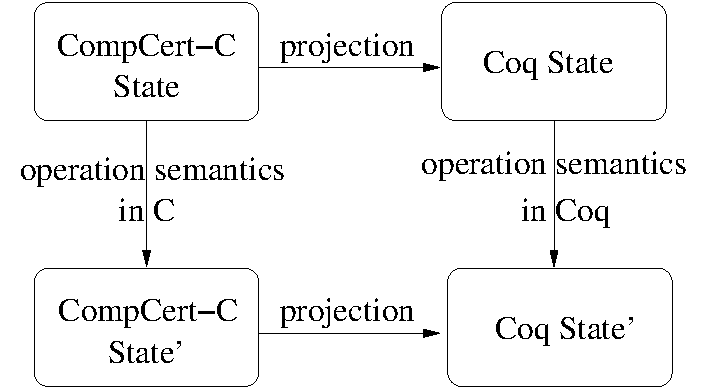
\includegraphics[width=.5\linewidth]{theorem.pdf}
\caption{Correctness of the simulation of an ARM operation}
\label{fig:thrm}
\end{figure}

% Using the CompCert defined operational semantics for program
% correctness proof requires quite a lot of interactive efforts. 
% For a system complicated like this, a full system simulation with a complete
% instruction set simulation, the specification is very detailed
% describing a processor state transistion system.  
% The theorem is stated relying on CompCert operational semantics.
The operational semantics of C defining the evaluation is used everywhere 
in the proof: it provides the decomposition of the vertical arrow
on the left column of Fig.~\ref{fig:thrm} 
and drives the proof accordingly. %  sequences steping forward.  
%
We use the big step semantics, 
which is defined in CompCert by 5 mutually inductive transition relations.
The largest inductive type for the evaluation of C expressions 
is \coqdocvar{eval\_expr}.
It has 17 constructors, one for each CompCert C expression 
such as assignment, binary operation, dereference, etc.  
% Since each ARM instruction operation is defined by a sequence of quite
% complex statements which can be decomposed into many single expressions.

% A typical proof step starts with an intuitive goal, 
% stating that a pair of C memory states are related 
% by one or several expressions. 
% To reveal the relation between the two memory states is the first target. 

In a typical proof step, 
we start from a goal containing 
a conclusion stating that 
a C memory state $m_n$ and an ARM state $st_n$ in the reference model 
are related by our projection,
a hypothesis $R_0$ stating a similar relation between 
a C memory state $m_0$ and an ARM state $st_0$,
and additional hypotheses $He_1, He_2, \ldots, He_n$.
relating pairs of successive C memory states 
$(m_0, m_1)$, $(m_1, m_2), \ldots, (m_{n-1}, m_n)$
respectively with (ASTs for) C expressions $e_1$, $e_2, \ldots,$ $e_n$,
according to the relevant transition relation provided by CompCert.
The general strategy is to propagate information
from $m_0$ to $m_1$ using $R_0$ and $He_1$, 
then so on until $m_n$.
To this effect we invert $He_1$, $He_2$, etc.
However, according to the structure of $e_1$, 
inverting $He_1$ generates intermediate memory states
and corresponding hypotheses that have to be inverted before 
going to $He_2$, unless $e_1$ is a base case.
And sometimes, other kind of reasoning steps are needed,
e.g., lemmas on the reference model of ARM.

% Then such hypothesis need to be inverted according
% to its inductively defined definition. 
% The result of inverting should either yields more permises 
% for these two memory state or finally
% tells the memory states are equivalent. 
% The new given permises could be again elementary transitions 
% between those states.  

% And the drawblack is very obvious here by using the Coq build-in tactic \inversion. 

%In detail,
%changes in the C memory model are formally described
%by a transition system according to the operational semantics of Compcert-C.
%Therefore, the later is  used everywhere in the proofs. 
%This operational semantics is described by
%a big mutual inductive type;
%in particular, the evaluation of expressions is defined by
%16 constructors, one for each CompCert C expression such as assignment or binary
%operation.
%% And this inductive type evaluation of expression is our target to try the
%% improved new inversion.
%A typical proof step starts from a goal intuitively saying that,
%given two C memory states related by a C expression,
%as expressed in some hypothesis $H$, 
%some commutative diagram holds.
%Then $H$ is inverted, which either yields more elementary 
%transitions between C memory states, 
%with corresponding expected commutative diagrams,

%or solves the current diagram if the considered expression
%is atomic. 
%In general we see that an inversion will result in many
%new opportunities to perform inversions.

%In our first proofs, using the Coq standard \inversion tactic
%resulted in a very weak control on the script.
%Finding the right relation to focus on in the hypotheses
%was inconvenient.
%Interactive execution of the script was also quite slow,
%due to the size of the terms generated by \inversion.
%And the compilation time for the proof on only one instruction 
%took more than one minute --
%there are more than one hundred instructions in the ARMv6 architecture.
%Moreover
%the proof code is fragile in case of changes: 
%after \inversion, hypotheses are automatically given similar names 
%according to a simple numbering scheme,
%so that any modification at the beginning of the proof script
%or in auxiliary lemmas 
%result in a complete renaming of hypotheses to come in the sequel.
%This is quite harmful in practice and constitutes
%a serious issue for maintenance.

For illustration,
the following code shows a small excerpt from an old proof script in
SimSoC-Cert using \inversion. 
It corresponds to one line taken in an instruction called ADC (add with carry).
It sets the CPSR (Current Program Status Register) with the value of SPSR 
(Saved Program Status Register). 
Lemma $same\_cp\_SR$ states that 
the C memory state of the simulator and 
the corresponding formal representation of ARM processor state 
evolve consistently during this assignment.
The pseudo-code from the ARM reference manual is just $CPSR~=~SPSR$.
The corresponding C code is represented by the identifier $cp\_SR$ 
in the statement of the lemma.

\coqdocinput{chunk43}

\medskip\noindent
After a couple of introductions and other administrative steps,
we get the following goal,  
where $cp\_SR$ is unfolded in hypothesis $H$.

%\coqdocinput{chunk45}

\medskip
\dots \\
\hspace*{-1.7mm}
\coqdocinput{chunk41}

\noindent
Then we have to invert $H$ and similar generated hypotheses
until all constructors used in it type are exhausted. 
Here 18 consecutive inversions are needed.
Using \inv, which performs standard \inversion, clearing 
the inverted hypothesis and rewriting of all auxiliary equations,
the sequel of the script started as follows.
% To make use of hypothesis $H$, We see inside the proof many \inv are
% used.  Here \inv denoted three proving tactics \coqdocvar{inversion H;
%   clear H; subst}: inverting the hypothesis, delete the useless
% original hypothesis, and substitutions.  We chose to use \inv tactics
% to save developement time without providing names and such combined
% tactic is easy to write.  Then the problem arrived, it is not possible
% to understand the proof just reading a list of \inv, even for the
% writer who wrote them a while ago.

\medskip
\coqdocinput{chunk42}
\medskip

\noindent
The names used there ($H4$, $H9$, etc.) are not under our control.
The program for simulating an ARM
instruction usually contains expression more complex than in the
example given here.
% This cumbersome work is needed in correctness proofs for every instruction,
And unfortunately there is no clear way to share parts of the proofs
involved since the corresponding programs are rather specific,
at least for instructions belonging to different categories.

The drawbacks of the standard tactic \inversion presented
in the introduction show up immediatly.
%
A first clue is the response time of Coq when inverting hypotheses $H_i$.
Compiling the proof script corresponding to one instruction
took more than a minute.
%
% Second, maintaining the proof scripts is harder than expected. 
% The proof code is fragile, 
% once a modification is required inside proving, from that point
% to the end the proof stradegy need to be modified all over again.
% Because applying the build-in \inversion itself will automatically
% name the new introduced elements. And the following script will refer
% to some of these names. 
%
% The naming algorithm of build-in \inversion just uses index for hypothesis, 
% then reading the code without any comments is not possible to understand the meaning of each step. 
% And a small modification may change the order of naming all the following
% hypotheses.  If we use \inversion with option, in order to have name
% controls, the other problem will be raised due to the size of the
% targeting inductive type of the hypotheses. 
%
% As we mentioned before,
% the inductive type which representing the evaluation has a lot of
% constructors which are all well-detailed.  
%
About the naming issue, 
the constructors we face have up to 19 variables and 6 premises,
yielding 25 names to provide.
We could try to automate this naming using an ad-hoc wrapper 
around \inversion, 
but things are complicated by 
the fact that this inversion program inserts
additional hypotheses putting equational constraints 
between variables of the inverted constructor.
There are different ways to state and to place such constraints,
and different releases of Coq may make different choices.
The BasicElim approach introduces equations as well
but from on our experiments, 
generated goals are much more regular than with \inversion.
In contrast, 
our approach does not suffer from such interferences,
so we are anyway in a better position. 

% Therefore, 
% inverting a hypothesis corresponding to this case yields 25 names to give.
% And due to the complexity of an expression. 
% Such \inversion with option of naming
% control need to apply for many times. Then giving names to 25 elements
% will be repeated for times. It is absolutly a very boring work.

% Then the hand crafted tactic should be able to deal with the two problem
% above, and also be robust enough against the changing of proof
% environment.  The following will detailed all the effort we have
% performed for SimSoC-Cert project rely on our ad-hoc inversion tactic
% presented in the last sections.

% Thanks to the technique introduced in this paper, we could define
% convenient reusable tactics. 
First, we define the diagonal-based function for each constructor 
of $eval\_expr$, following the lines given in the previous section.
For example, 
the evaluation of a field is defined in CompCert by the following rule.

\medskip
\coqdocinput{chunk50}
\medskip

\noindent
We then define (observe that 2 variables and 1 hypothesis will be generated):

\medskip
\coqdocinput{chunk52}
\medskip

% An interesting one, for expression $val\_of$, 
% has it inversion function defined as follows.
%
% \medskip
% \coqdocinput{chunk40}
% \medskip
%
% % It is fully depended on the constructor $eval\_valof$ definition. The
% % implicit arguments of $inv\_valof$ are the references helps us to
% % indicate the the object hypothesis. 
% $inv\_valof$ is special, because the memory access can be volatile or not,
% so that inverting the hypothesis of type $eval\_valof$ returns two cases,
% whereas we get only one case for all other constructors.
% Using the impredicative encoding here in the diagonal function
% can achieve the same casing effect. If type of the expression is
% volatile, we have to evaluate such expression again to get the
% reduction result, then ask for the volatile type to perform the same
% process all over.

%Thanks to the technique introduced in this paper,
%we could define convenient reusable tactics.
%First, we defined suitable diagonal-based functions for each
%constructor of $eval\_expr$ following the lines given in the
%previous section.

% As we showed in the example above, the old way of inverting hypotheses is a 
% repetitive work. To get the relation of memory states between a not too
% complex expression requires 18 \inv. 
% After we changed to the new inversion,
% we still need 18 corresponding ad-hoc inversions for every decomposed
% expression.
Next we introduce a high-level tactic 
% aiming such problem happened in SimSoC-Cert project. 
for each inductive type, gathering all the functions defined for 
its constructors. % and solve the heavy and repetitive naming trouble. 
For example, $eval\_expr$ contains:

\medskip
\coqdocinput{chunk51}

\noindent
This tactic has two arguments $m$ and $m'$, corresponding to C memory states.
The first \texttt{intros} introduces the 3 generated components 
with names respectively prefixed by \coqdoccst{t}, \coqdoccst{v} and \coqdoccst{ev\_ex}.
The second \texttt{intros} is related to previously reverted 
hypotheses, their names are correctly managed by Coq.
Alltogether, such a tactic will:
\begin{enumerate}
\item Automatically find the hypothesis matching the arguments to be inverted;
\item Repeatedly perform our hand-crafted inversions for type
  $eval\_expr$ until all constraints between two memory states $m$ and
  $m'$ are derived;
\item Give meaningful names to the derived constraints;
\item Update all other related hypotheses according to the new 
  variable names or values;
\item Clean up useless variables and hypotheses.
\end{enumerate}
%

%Then we packaged them together in a high-level tactic named 
%$inv\_eval\_expr$ using an Ltac definition. The arguments of this
%tactic are the memory states under focus --
%in the example above: $m$ and $m'$.
%This tactic also contains extra features so that
%it is able to:
%%
%\begin{enumerate}
%\item automatically find an hypothesis to be inverted;
%\item repeatedly perform our hand-crafted inversion until all constraints
%  between two memory states are derived;
%\item give meaningful names to the derived constraints;
%\item update all other related hypotheses according to the new 
%  variable names or values;
%\item clean up useless variables and hypotheses.
%\end{enumerate}
%%
\noindent
For example the 18 \inv in the example above are solved in 
one step using $inv\_eval\_expr~m~m'$, 
Note that the names are not explicitly given in the script,
which would be cumbersome,
but generated in our tactic.

% Defining such high-level tactics is aim to avoid repetitively naming issue
% we mentioned, the real killer in our developement of correctness proof.
% Like constructor $eval\_valof\_volatile$ in type $eval\_expr$ requires 17
% names to give if we want this full control. 
% Using the ad-hoc tactics like $inv\_eval\_expr$ requires no name to
% give to variables or hypotheses.The names are given during defining
% %the general hc\_inversion, according to the meaning of the hypo
% %orwhatever names you can recognise later.For example, hypo
% the general \verb!hc_inversion!, \todo{a}{newcommand for hcinv}
% according to the meaning of the hypothesis
% or whatever names you can recognise later. 
% For example, hypothesis
% $find\_funct~ge~vf$ is named $Hfindfunc$. When maintaining the scripts,
% we know which hypo it refers to. It is done once for all. Unlike using
% build-in inversion, you don't need to look at the big inductive
% definition for the long list of variables and premises every time you
% apply inversion. The naming stradegy used in this kind of high-level tactic
% is semi automatic. We can have a better control by giving names according to
% the type of the hypotheses. But the names of hypotheses of the same type will
% be named with index at the end $Hfindfunc1$ $Hfindfunc2$. We have to compromise
% between making the tactic easy to apply with and even a better control on index.
% Here we prefer the tactic to be simple and easy to use.

% \todo{r}{BEGIN to be removed -- or moved to intro}%
% To be fair, let us mention that the robustness issue could,
% in principle, be managed using the current version of standard \inversion,
% because it allows us 
% to give explicit names to introduced variables and hypotheses.
% However, due to the complexity of CompCert C semantics, 
% providing all these names explicitly turns out to be cumbersome,
% and unrealistic when you face dozens of consecutive \inversion 
% and about ten names for each \inversion.
% \todo{r'}{END to be removed -- or moved to intro}%
% Within our framework,
% the introduction of suitable names
% is automatically performed inside $inv\_eval\_expr~m~m'$.
% Names are chosen according to the contents and in a flexible way, 
% so that the evolution of goals is easy to follow.

Coq version changes had no impact on our scripts.
Unexpectedly, 
changes in CompCert C semantics between versions 1.9 and 1.11
had no impact as well on proof scripts using our inversion.
Of course, we still had to update the definition of diagonal functions. 
% In the proof script, the step for inverting on an inductive type will
% always uses its specific ad-hoc inversion without any change. 
% But the changes in the script may happen, if the following step refers to
% some new derived elements.

Comparing development times provides additional hints.  
In our first try, using built-in inversion,
more than two months were spent (by one person) on the development of 
the correctness proof of instruction ADC.
Much time was actually wasted at maintaining the proofs since,
as mentioned, a little change resulted in 
a complete revision of proof scripts. 
% That's one of the important argument we need this ad-hoc inversion to be apply in SimSoC-Cert project.  
We then designed the inversion technique presented here.
% was not available at that time, entailing the drawbacks detailed above.  
With the new approach, proofs for 4 other simple instructions 
could be finished in only one week, 
taking of course advantage of the previous experience with ADC.
The high-level tactic described above required less than 2 weeks.

Finally, let us compare the efficiency of Coq built-in inversions 
(\inversion, 
\derive \inversion which can generate an inversion principle once for all, 
and BasicElim~\cite{mcbride00}) with our inversion.
We apply the four methods to the same examples, the lemma $cp\_SR$ and
a single inversion on type $eval\_expr$ from CompCert C semantics.
% Finally, we compare the efficiency of the standard Coq \inversion with
% our new tactic in Table.~\ref{t:timing}.  
The first row is about the whole expression given in the example above. 
The other rows are inversions of specific expressions: 
$Ecall$ is the CompCert-C expression of function calls, 
$Evalof$ is to get the value of the specified location, 
$Eval$ is to express constant, and $Evar$ is to express variables.  
We can observe a gain of about 4 to 5 times.
And generated object files are 5 times smaller.
%And compilation generates object files which are 5 times smaller.

% Finished transaction in 1. secs (1.428089u,0.024001s)
% Finished transaction in 0. secs (0.31202u,0.s)
% Finished transaction in 2. secs (1.628102u,0.s)
% Finished transaction in 1. secs (0.976061u,0.020001s)


\begin{table}\centering
\label{t:timing}
\caption{Time costs (in seconds)}
\begin{tabular}{|l|c|c|c|c|}
\hline
 & standard \inversion & \derive \inversion & BasicElim & our inversion \\
\hline
%Full example & 1.628102 & 0.976061 & 1.428089 & 0.31202 \\
Full example & 1.628 & 0.976 & 1.428 & 0.312 \\
\hline
%Ecall & 0.132009 & 0.076004 & 0.112007 &  0.028002\\
Ecall & 0.132 & 0.076 & 0.112 &  0.028\\
\hline
%Evalof &  0.132008 & 0.072004 & 0.092005 & 0.020001\\
Evalof &  0.132 & 0.072 & 0.092 & 0.020\\
\hline
%Evar &  0.128008 & 0.064004 & 0.084006 & 0.024001\\
Evar &  0.128 & 0.064 & 0.084 & 0.024\\
\hline
%Eaddrof &  0.140009 & 0.076005 & 0.104007 & 0.020001\\
Eaddrof &  0.140 & 0.076 & 0.104 & 0.020\\
\hline
\end{tabular}
\end{table}

% -rw-rw-r-- 1 xiaomu-shi xiaomu-shi  36712 Feb  5 19:50 comparison_ahinv.vo
% -rw-rw-r-- 1 xiaomu-shi xiaomu-shi 170821 Feb  5 19:50 comparison_basicelim.vo
% -rw-rw-r-- 1 xiaomu-shi xiaomu-shi 191346 Feb  5 19:50 comparison_inv.vo
% -rw-rw-r-- 1 xiaomu-shi xiaomu-shi 459613 Feb  5 23:40 comparison_derinv.vo


\begin{table}\centering
\label{t:size}
\caption{Size of compilation results (in KBytes)}
\begin{tabular}{|l|c|c|c|c|}
\hline
 & standard \inversion & \derive \inversion & BasicElim & our inversion \\
\hline
%Full example & 191346 & 459613 & 170821 & 36712\\
Full example & 191 & 460 & 171 & 37\\
\hline
\end{tabular}
\end{table}

%%% Local Variables: 
%%% mode: latex
%%% TeX-master: "itp13"
%%% End: 

\svnidlong
{$HeadURL: https://scm.gforge.inria.fr/anonscm/svn/simsoc-cert/papers/itp13/conclusion.tex $}
{$LastChangedDate: 2013-04-17 11:55:45 +0200 (Wed, 17 Apr 2013) $}
{$LastChangedRevision: 2298 $}
{$LastChangedBy: monin $}

% Author: \svnfileauthor; Revision: \svnfilerev; Last changed on: \svnfiledate; 
% URL: \url{\svnkw{HeadURL}}

\begin{thoughts}
\itshape
\hfil -----------------------------------------------------------------------------------\par
\hfil \textbf{Changes on \currfilename}

Author: \svnfileauthor; Revision: \svnfilerev; Last changed on: \svnfiledate
\end{thoughts}

% svn propset svn:keywords 'LastChangedBy LastChangedRevision LastChangedDate HeadURL' thisfile.tex

%%%%%%%%%%%%%%%%%%%%%%%%%%%%%%%%%%%%%%%%%%%%%%%%%%%%%%%%%%%%%%%%%%%%%%%%%%%%%
\section{Conclusion}
\label{sec:conclusion}


We see no reason why
the technique developed above for performing inversions could not
be automated and implemented in Coq or in proof assistants
based on a similar calculus.
One good motivation for that would be to get terms which are 
much smaller, easier to typecheck,
than with the currently available inversion tactics.
This can be very useful when interactively defining functions
on dependent types, for instance. %\todo{a}{manual already useful there indeed}

But we want to insist first on a much more important feature of
our approach, according to our experience with SimSoC-Cert:
its impact on goals during \emph{interactive} proof development
is \emph{actually controllable}.
We think that having much shorter underlying functions is
helpful in this respect:
they are short enough to be written by hand,
providing an exact view on what is to be generated.
We claim that this feature is especially relevant
to applications which make an intensive use of inversion steps:
in this situation, 
partial automation obtained by programming small controllable building blocks
turns out to be effective,
whereas automation tends to generate a 
response of the proof assistant which is not completely predictible. 
This may not harm too much if the generated goals can be fully discharged
without further interaction,
but this is not the general case.
In particular, this hope is vain when we deal with complex properties,
as in our application.
A better alternative would be to automatically generate 
auxiliary definitions such as \coqdocvar{inv\_field}.
However, we consider that our technique is already useful
and worth to be offered.

In contrast to available techniques \cite{cornes95automating,mcbride00}
we argue against the use of auxiliary equations or disequations:
the latter are better to be cleaned, 
in order to avoid clumsy additional hypotheses, 
which hamper the management of proof scripts;
however, it is not that simple to do.
The brute use of a tactic which performs all possible rewriting
steps, then cleans equalities avalaible in the goal, for instance, 
is not satisfactory
because some equalities already introduced by the user on purpose
could then disappear. 
Therefore, a special machinery is needed in order
to trace equalities coming from the inversion step under consideration
(e.g., the use of \coqdocvar{block} in BasicElim).
Our use of CPS encoding of Leibniz equality, on the other hand,
completely avoids this issue.

Our method was experimented on large proofs relying on 
big inductive relations independently defined in the Compcert project.

The current development can be found on-line~\cite{hci:examples},
as well as examples given in Section~\ref{sec:hci}.

Our group recently started another project dedicated
to a certifying compiler from a high-level component-based language dedicated
to embedded systems (BIP), with CompCert C as its target. 
We expect the work presented here and our high-level tactics
to be reused there.

Let us mention another possible application of the technique.
Inversion is sometimes
needed to write a function whose properties will be established later (as
opposed to providing a monolithic and exhaustive Hoare-style specification and
along with a VC generator such as Program). 
In this context simply using the proof engine and the \inversion tactic
tends to generate unmanageably large terms.
We expect our technique to be very helpful in such situations.


%%% Local Variables: 
%%% mode: latex
%%% TeX-master: "itp13"
%%% End: 



\bibliographystyle{abbrv}
\bibliography{biblio}

\end{document}


%-------------------------------------------------------------------------


%%% Local Variables: 
%%% mode: latex
%%% TeX-master: "cpp12"
%%% End: 
